\documentclass{article}[a4]
\usepackage[utf8]{inputenc}
\usepackage{authblk}
\usepackage{tabularx}
\usepackage{url}
\usepackage{verbatimbox}
\usepackage{graphicx}
\graphicspath{{images/}}

\title{Proposal of Automatic Extraction Framework of Superconductors related Information from Scientific literature}

\author[1]{Luca Foppiano\thanks{FOPPIANO.Luca@nims.go.jp}}
\author[1]{Thaer M. Dieb\thanks{MOUSTAFADIEB.Thaer@nims.go.jp}}
\author[1]{Akira Suzuki\thanks{SUZUKI.Akira3@nims.go.jp}}
\author[1]{Masashi Ishii\thanks{ISHII.Masashi@nims.go.jp}}
\affil[1]{Research and Services Division of Materials Data and Integrated System (MaDIS), National Institute for Materials Science (NIMS), 1-2-1 Sengen, Tsukuba, Ibaraki 305-0047, Japan}

% \date{April 2019}

\begin{document}

\maketitle

\begin{abstract}
Automatic collection of materials information from research papers using natural language processing is highly required for rapid materials development using big data, namely materials informatics (MI). Difficulty of this automatic collection is mainly caused by the variety of expressions in the papers, a system with tolerance to such variety is required to be developed. 
In this paper, we report an ongoing interdisciplinary work to construct the system for automatic collection of superconductor-related information from scientific literature using text mining techniques. We focused on identification of superconducting materials and their key property of critical temperature (Tc), and discussed machine learning (ML) techniques, including annotation strategies to obtain appropriate training data. We introduce a guideline for the annotation together with our several trails of ML on subsequent automatic data collection.
\end{abstract}

%% The table of content is there just for organisation purposes, will be removed 
\pagebreak

% \tableofcontents

% \pagebreak

%Research in superconductors is always articulated over two main axes, finding new conditions or discovering new materials (or combination of it) show new or better superconductivity properties. 
%In order to do so, material scientists needs to have rapid access to materials known to be superconductors and their properties without have to examine the thousand of papers related to it. Such data can also be used by further systems to compute generative models 


\section{Introduction}
% What is the problem we are trying to solve? What are the motivation behind this project? 

Automatic extraction of information from research papers using Natural Language processing is a highly required approach in many domains. In material research, the utilisation of large available of experimental data can give insight leading to new break-trough in materials discovery. Large availability of scientific papers and the expertise costs for manually generated such data justify the needs of Text and Data Mining automatic approaches.

Diverse writing style, variability in experiment and result description are just two of the variables making this task particularly complex.


%% How research is made and what are the point of improvements?
\textit{Superconductivity is a phenomenon of exactly zero electrical resistance and expulsion of magnetic flux fields occurring in certain materials, called superconductors, when cooled below a characteristic critical temperature.}\footnote{\url{https://en.wikipedia.org/wiki/Superconductivity}}

Historically, high-temperature superconductors were suddenly improved not mainly modifying the existed materials but finding new materials because of the lack of theoretical understanding \cite{klintenberg2013possible} \cite{DBLP:journals/corr/abs-1812-01995}. Data-driven exploration \cite{doi:10.1080/14686996.2018.1548885} \cite{HAMIDIEH2018346}\cite{PhysRevMaterials.2.024802}\cite{doi:10.1021/cm503507h} would be an optimal approach to accelerate development of new superconducting materials. However, it is required to prepare huge data sets for the prediction by high-throughput experiments or first-principle calculations and existing material databases. Currently there are several general material databases available, however when looking at the superconductor sub-domain the main one is SuperCon\cite{SuperCon}. Hosted and maintained by the National Institute for Materials Science (NIMS) containing about 32k inorganic and about 558 organic superconductor material definitions. Although it is being updated manually, it can not catch up with the massive fresh information from the increasing number of articles each year. It is our challenge to make SuperCon more content oriented to data-driven science by automatically extracting superconductors related Information from scientific literature using text mining techniques.

%The research in superconductor materials is articulated toward many different objectives. Discovery of new characteristic of well known materials, under new environment condition, like applied pressure or magnetic field. Combination of known superconductors with non-superconductors may lead to new materials with better characteristics, usually a higher critical temperature. 

% Add that introduction about the available databases, in particular NIMS, which has the problem that is not updated due to high costs of manual work
%Currently there are several general material databases available, however when looking  at the superconductor sub-domain the main one is SuperCon\cite{SuperCon}. Hosted and maintained by the National Institute for Materials Science (NIMS) containing about 32k inorganic and about 558 organic superconductor material definitions. Although the update continues manually, the latest information can not keep up with the increase in the enormous number of articles each year. 

% Why do we need such information? Why these information are important?
%The availability of material information with detailed and precise granularity is a must-have for superconductors scientists. This data summarises decades of research and discoveries and can be potentially exploited in many areas. Machine learning or neural models can train generative models specialised in automatically predict critical temperature \cite{DBLP:journals/corr/abs-1812-01995} on new (pure or intercalated) materials. Large scale repositories with enhanced search specialised in semantic superconductor disambiguation, document recommendation, and so on. 

In this paper we describe the ongoing attempt to design a system aiming to automatically extract superconductor-related information from scientific literature based using Natural Language Processing techniques. In particular, we focus on extracting materials names linking it with they corresponding critical temperature (Tc) values.
Our system is built on an Open Source library for text mining from scholarly documents: Grobid \cite{GROBID}. We evaluate the performance of the system using precision, recall and f-score. Such preliminary results are considered as our baseline for measuring our progress in solving the task.
Similar attempts of mining scientific literature in materials domain had been conducted  \cite{nanocrystal_extraction}, \cite{court2018auto}. 

% What we discuss in this paper? 
This paper is organised as follows, Section \ref{sec:architecture} describes the development of a working prototype specialised in superconductors data extraction including the development of an annotated corpus for material names recognition. Section \ref{sec:experiments-results}  presents the evaluation experiment and discuss the results, while section \ref{sec:conclusion}  concludes the paper.

\section{System architecture}
\label{sec:architecture}
In collaboration with superconductor domain experts, we discussed the relevant information and their use in research activities. Depending on the writing style, these information are often presented as tables and plots as they summarise more effectively giving quicker understanding to a human reader. In order to achieve high quality and consistency of the extracted information, it is necessary to link the extracted entities. For example, the superconductivity differs in expression and property values depending on the difference in composition due to impurity effects, or on the pressure and magnetic field conditions. In such a case, linking the critical temperature (Tc) with its corresponding superconducting material is crucial. In the scope of this paper, we focus on information exist in the main body text and in captions (tables and figures). Other properties will be targeted in the upcoming work.


% I think this reason is not good
% Among all, T\textsubscript{c} plays a critical role because is the reference property in superconductor research. For this reason, in the scope of this paper, we focus on extracting material names with their corresponding critical temperature. 

We build our implementation based on an open source library called GROBID \cite{GROBID}. GROBID is a sequence labelling and document segmentation originally based on Machine Learning algorithm Conditional Random Field (CRF) \cite{lafferty2001conditional}. It provides full support for extraction of data from PDF and a build-in workflow for pre-annotating training data, evaluation and training. 
The PDF support in GROBID was important because allowed us to work with a “standardised” format instead of dealing with several flavour of XML formats, on the other hand having to deal with PDF noise made our attempt more realistic in a real word scenario. Among different similar open source tools available, the choice of GROBID is well justified by the fact that it's still actively developed and it's a production ready product deployed in the back-end of Mendeley \cite{mendeley-extraction} and other research repositories. GROBID performed best in a recent benchmark testing for citation extraction \cite{DBLP:journals/corr/abs-1802-01168}. Lastly, GROBID has been successfully extended to support several domains specific problems, for example astronomical entities recognition \cite{grobid-astro}, dictionaries segmentation \cite{khemakhem2017automatic}, software mention \cite{software-mentions} and measurements extraction and normalisation \cite{grobid-quantities}. The availability of an open source measurement recognition like Grobid-quantities was fitting perfectly for our use case to recognise temperatures. 

\begin{figure}[]
    \centering
    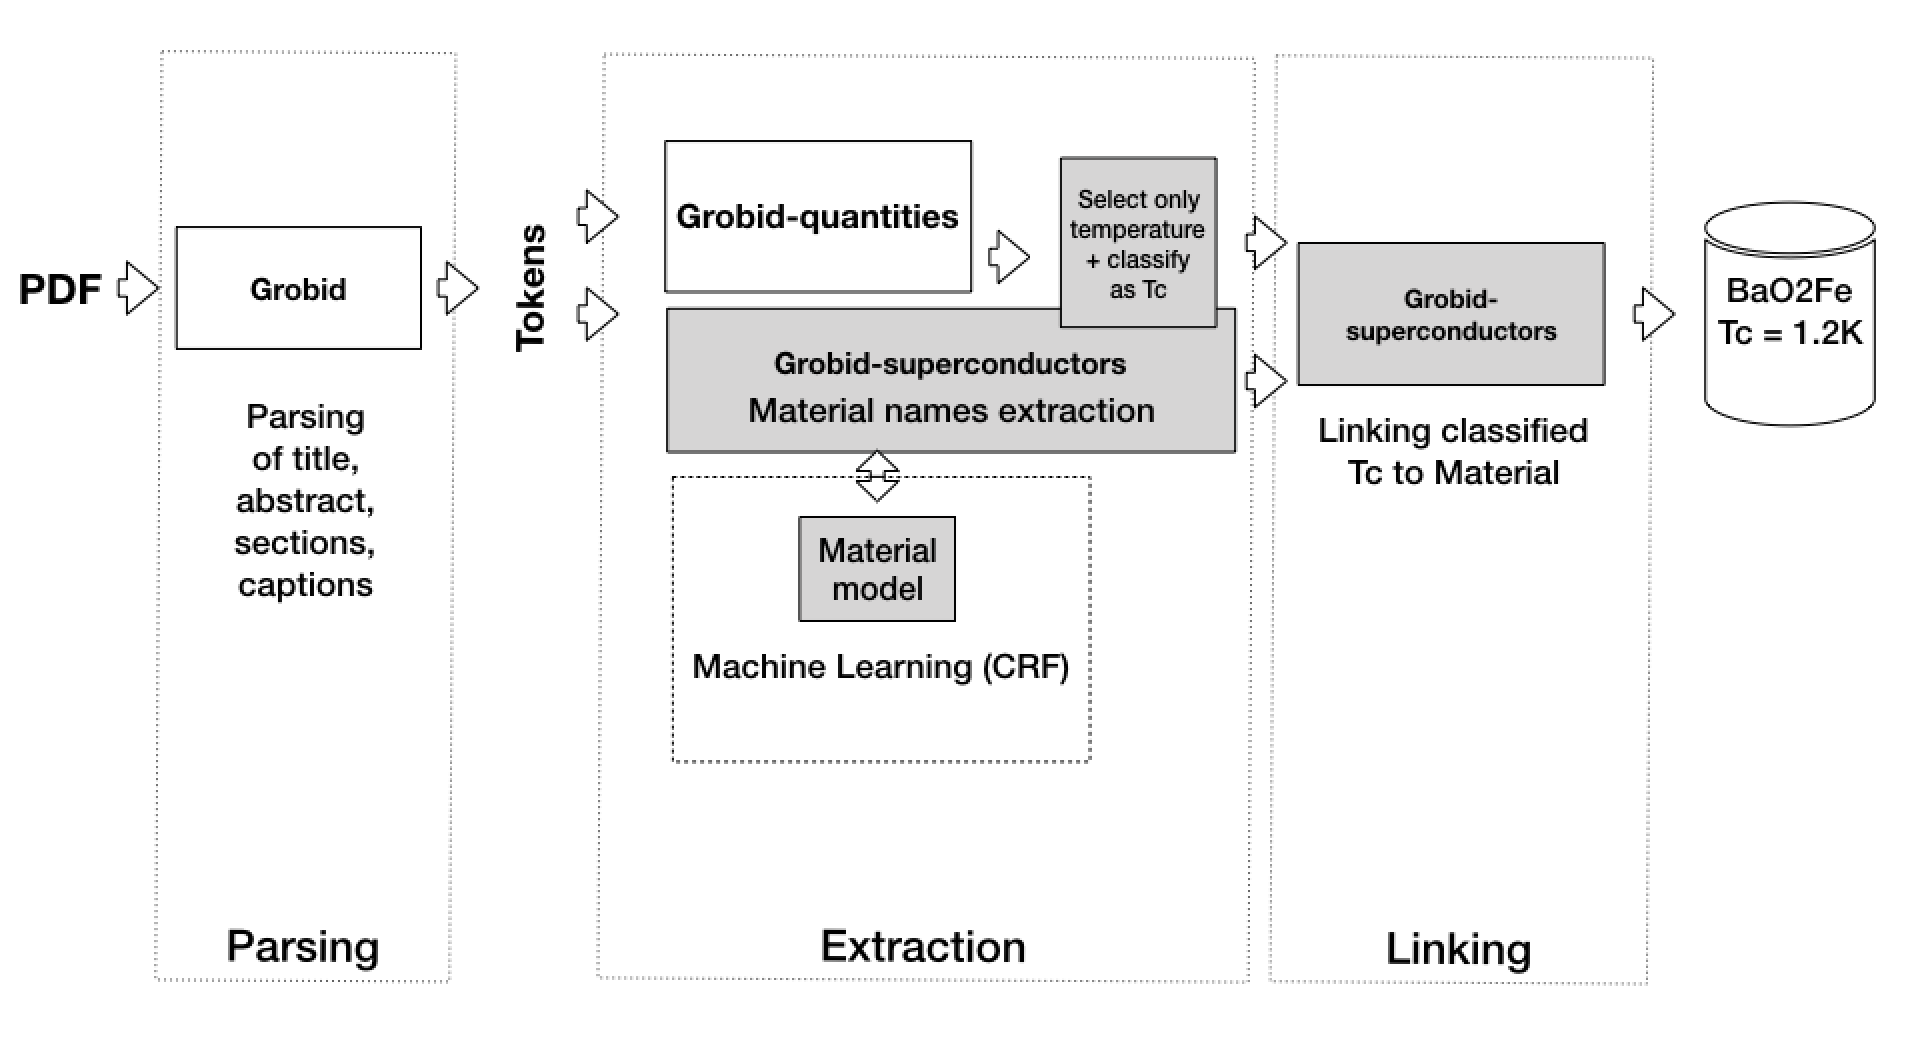
\includegraphics[width=4in]{schema}
    \caption[Schema of the system] {Schema of the system}
    \label{fig:system-schema}
\end{figure}

Our system can be decomposed in two phases: first we extract relevant entities (materials and temperatures) and second, we link the critical temperatures to their corresponding superconducting materials. Figure \ref{fig:system-schema} illustrates the outline of the proposed system. 

The extraction phase combines the entities resulting from a newly trained model for superconductor material recognition and an existing module, Grobid-quantities for measurement extraction, parsing and normalisation. The superconductor material model was trained with 5 full documents (42 mentions in total) manually annotated. We added some specific features using a chemical extraction recogniser, called ChemSpot \cite{10.1093/bioinformatics/bts183}. ChemSpot provides classification of the extracted entities (FORMULA, SYSTEMATIC, COMPOUND). 

For the linking phase, three tasks are performed: since GROBID-quantities returns a larger set of measurements (temperatures, lengths, pressures, etc.) we selected only temperatures, then we classified each of them as "Critical Temperature" or "not Critical Temperature" and we linked each material term with the closest Tc. 
The process of classifying a temperature as Tc consisted in matching within a list of trigger words commonly used in superconducting literature (like “Tc” or “critical temperature”) within a window of 20 tokens around the temperature mention. We assumed that given a temperature value, the terms suggesting that is a Tc are located within 5 words from the temperature itself. Finally the link to a material was performed iterating on the materials and selecting the closest. The distance was measured as the distance between the centroid of the material (central offset) to the centroid of the temperature.
This simple algorithm allowed us to quickly develop a prototype implementing the end to end process and showing annotations directly in PDF or storing them in a database. In Figure \ref{fig:example-working} we show two examples of a correct linking, while in Figure \ref{fig:example-not-working} two example of incorrect linking or missing extraction. 

\begin{figure}[h]
    \centering
    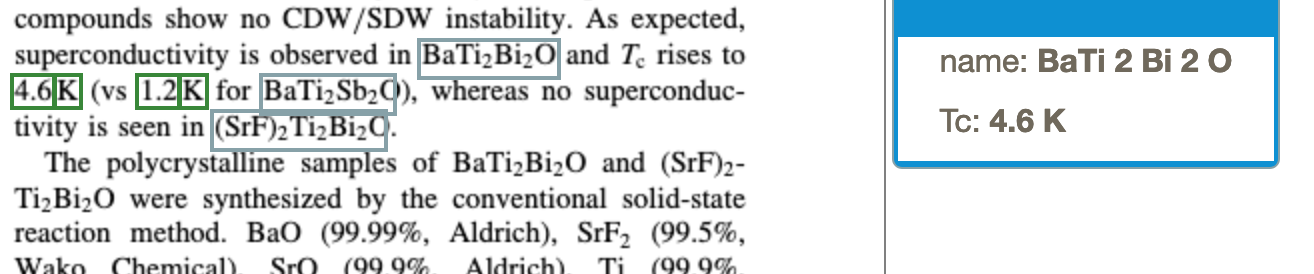
\includegraphics[width=4in]{example1} 
    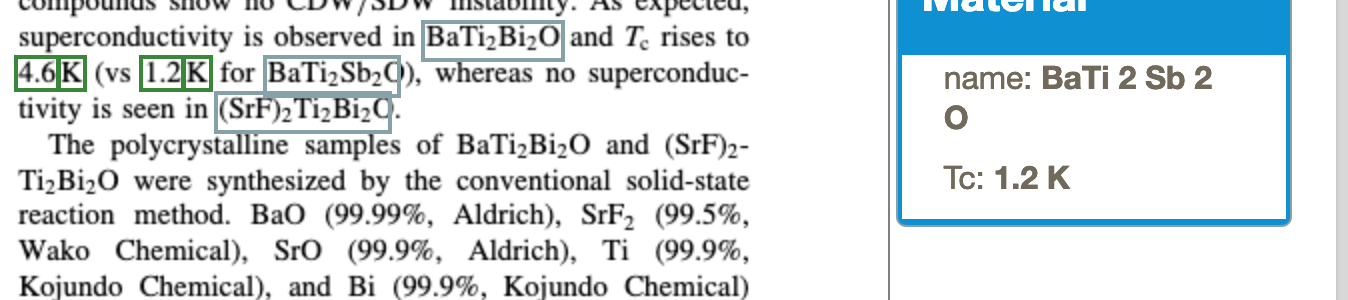
\includegraphics[width=4in]{example2}
    \caption{Example of a correct linking between material and Tc. First image is referring to the link between the material BaTi\textsubscript{2}Bi\textsubscript{2}O with 4.6K and BaTi\textsubscript{2}Sb\textsubscript{2}O with 1.2K}.
    \label{fig:example-working}
\end{figure}

\begin{figure}[h]
    \centering
    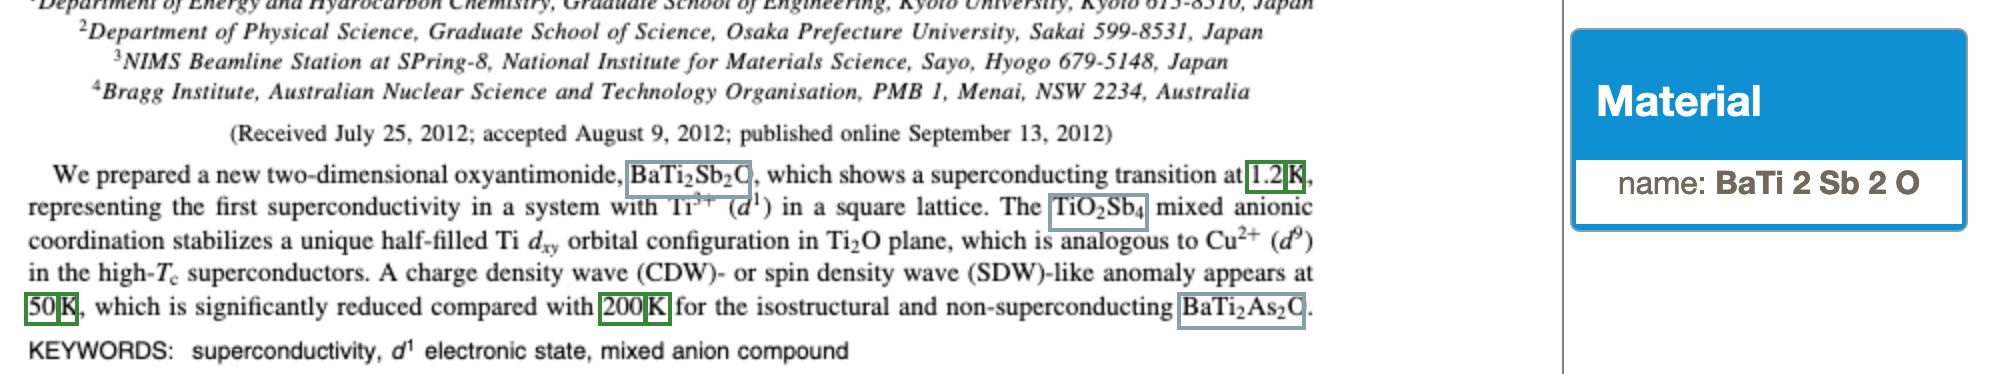
\includegraphics[width=4in]{example-bad1} 
    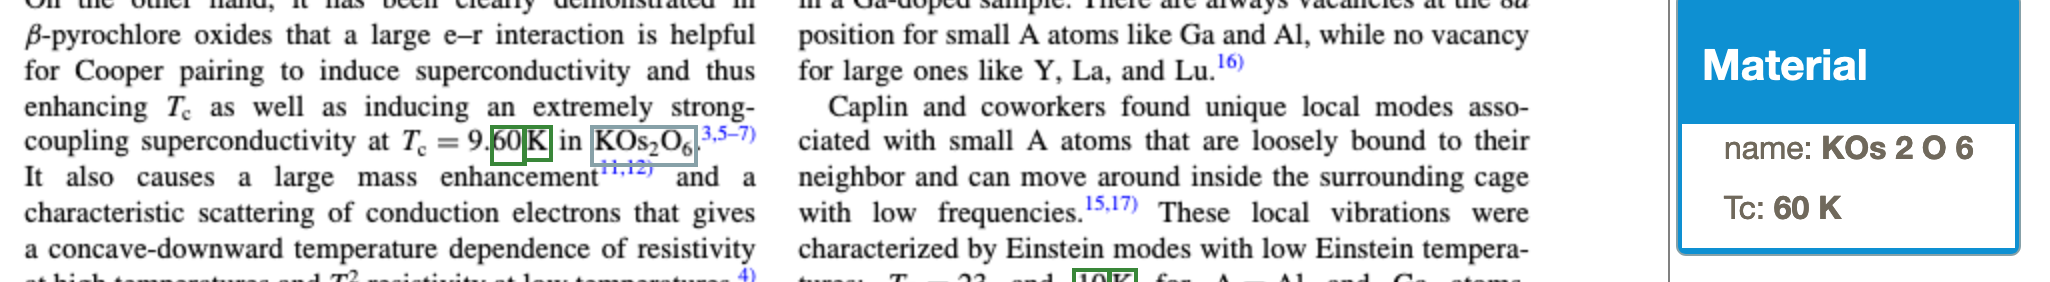
\includegraphics[width=4in]{example-bad2}
    \caption{Example of a incorrect linking between material and Tc. In the top example the link is correctly performed but the critical temperature is extracted incorrectly. The bottom show a missing link due to incorrect classification of critical temperature.}
    \label{fig:example-not-working}
\end{figure}

\section{Experiments and results}
\label{sec:experiments-results}

In this section we discuss a preliminary evaluation for the superconductor model  and some consideration on results on a larger corpus. We conclude this section by discussing use cases in which the rule base approach doesn't perform well. 

The superconductor model was trained using a corpus of 5 papers (4 for training and 1 for evaluation) having a total of 42 entities classified with a single label called  \textless supercon\textgreater.

In GROBID evaluation framework the measures (accuracy, precision and recall) are calculated at three different levels: tokens-level, field-level and instance-level. 
Evaluation at token-level is computed considering each token independently, field-level consider each continuous sequence of the same label (a field, a sequence) belonging to the same labelled chunk. The more sophisticated result, at instance-level is the score for the whole input, for instance a paragraph.

The output from GROBID is shown in the following listing: 

\begin{verbnobox}[\small]
===== Token-level results =====

label                accuracy     precision    recall       f1     

<supercon>           98.61        84.42        85.28        84.85  

all fields           98.61        84.42        85.28        84.85   (micro average)
                     98.61        84.42        85.28        84.85   (macro average)

===== Field-level results =====

label                accuracy     precision    recall       f1     

<supercon>           72.94        66.67        56.25        61.02  

all fields           72.94        66.67        56.25        61.02   (micro average)
                     72.94        66.67        56.25        61.02   (macro average)

===== Instance-level results =====

Total expected instances:   22
Correct instances:          15
Instance-level recall:      68.18
\end{verbnobox}

While token-level f1-score is above 80\%, at field-level the f1-score is about 60\%. This difference (of about 20\%) in token and field level can be attributed to lack of training data, in fact the model is not yet able to generalise properly and fails especially on the edges of the entities. 
On the other hand the instance-level (corresponding to paragraph) are around 70\%, looks high considering the amount of training data supplied to the training. We can explain this as lack of variability of the training examples. 

%% Working on this set of results 

% On a more larger scale, we experiment the extraction from a corpus of 500 PDF superconductors papers from three publishers: AIP, APS and IOP. The system extracted 5400 materials, however only 76 were linked to a critical temperature. We manually verified all of them and found out that 50 were correctly linked. 
On a more larger scale, we experiment the extraction from a corpus of 500 PDF superconductors papers from three publishers: AIP, APS and IOP as summarised in Table \ref{table:result-extraction} where the linked materials were evaluated manually. 

\begin{table}[h!]
    \centering
    \begin{tabular}{ | m{4em} | m{4em} | m{6em} | m{5em} | m{3em} | m{4em}| } 
    \hline
        Material entities & Unique material entities & Temperature entities & Tc entities & Links & Correct links  \\
    \hline
        5400 & 1644 & 7554 & 1173 & 76 & 50 \\ 
    \hline
    \end{tabular}
    \label{table:result-extraction}
    \caption{Result of extraction on a corpus of 500 papers and comprehend unique material terms, mention of temperatures and Tc (after being classified). Finally we display total and correct amount of links between material and Tc.}    
\end{table}

The results of the linking process show high precision and very low recall. This was expected having implemented a Rule Base Approach (50/76 correct matches). There are several reason to explain these results, first of all we were processing PDfs, which, in several cases but not all, deliver high amount of noise (missing UTF-8 characters, flow ordering issues, fonts. etc.). Note that varieties of chemical compositions increase the number of the material entities. Temperatures could refer to experimental conditions or heat processes of specimen fabrication. It would be required to reduce noise and clustering terms before processing in TDM. Secondly the linking was performed on data carrying out relevant amount of errors from previous processing, which penalised the end results. 




\section{Conclusion}
\label{sec:conclusion}
In this paper, we introduced a proposal for automatic extraction of superconductor related information from related scientific publications using Sequence labelling. We report recall that suggests the Sequence labelling is promising.

The linking using Rule Based approach has shown relatively low tolerance to noise, for two main reasons: firstly the data extracted from PDF is generally not clean having characters wrongly extracted. Secondly, there were cases where the material name or the critical temperature was not explicitly recognised due to complex writing style.
We plan to experiment the following solutions: 1) improve the current approach adding more rules 2) implement a simple CRF model that allows the linking of relatively closed entities, and 3) study the possibility to exploit a sentence dependency parsing, bearing in mind the impact in performances should also be considered.

In the next step, we plan to test the system using Bi-LSTM+CRF approach based on deep learning and embeddings in collaboration with the domain experts. Increasing the size of the corpus is crucial for such testing. 



% Future works
% 
% \listoffigures
\pagebreak

\bibliography{references}
\bibliographystyle{plain}

\end{document}
